\ifpdf
\graphicspath{ {Chapters/Introduction/Figs/} }
\section{Theoretical Motivation}
\subsection{Proton Structure}
%\begin{frame}[label=current]

\begin{frame}
  \frametitle{Proton Structure}

  \begin{equation*}
     \sigma
  \end{equation*}
  
  \begin{columns}
    \column{0.4\textwidth}
    \begin{figure}
      \centering
      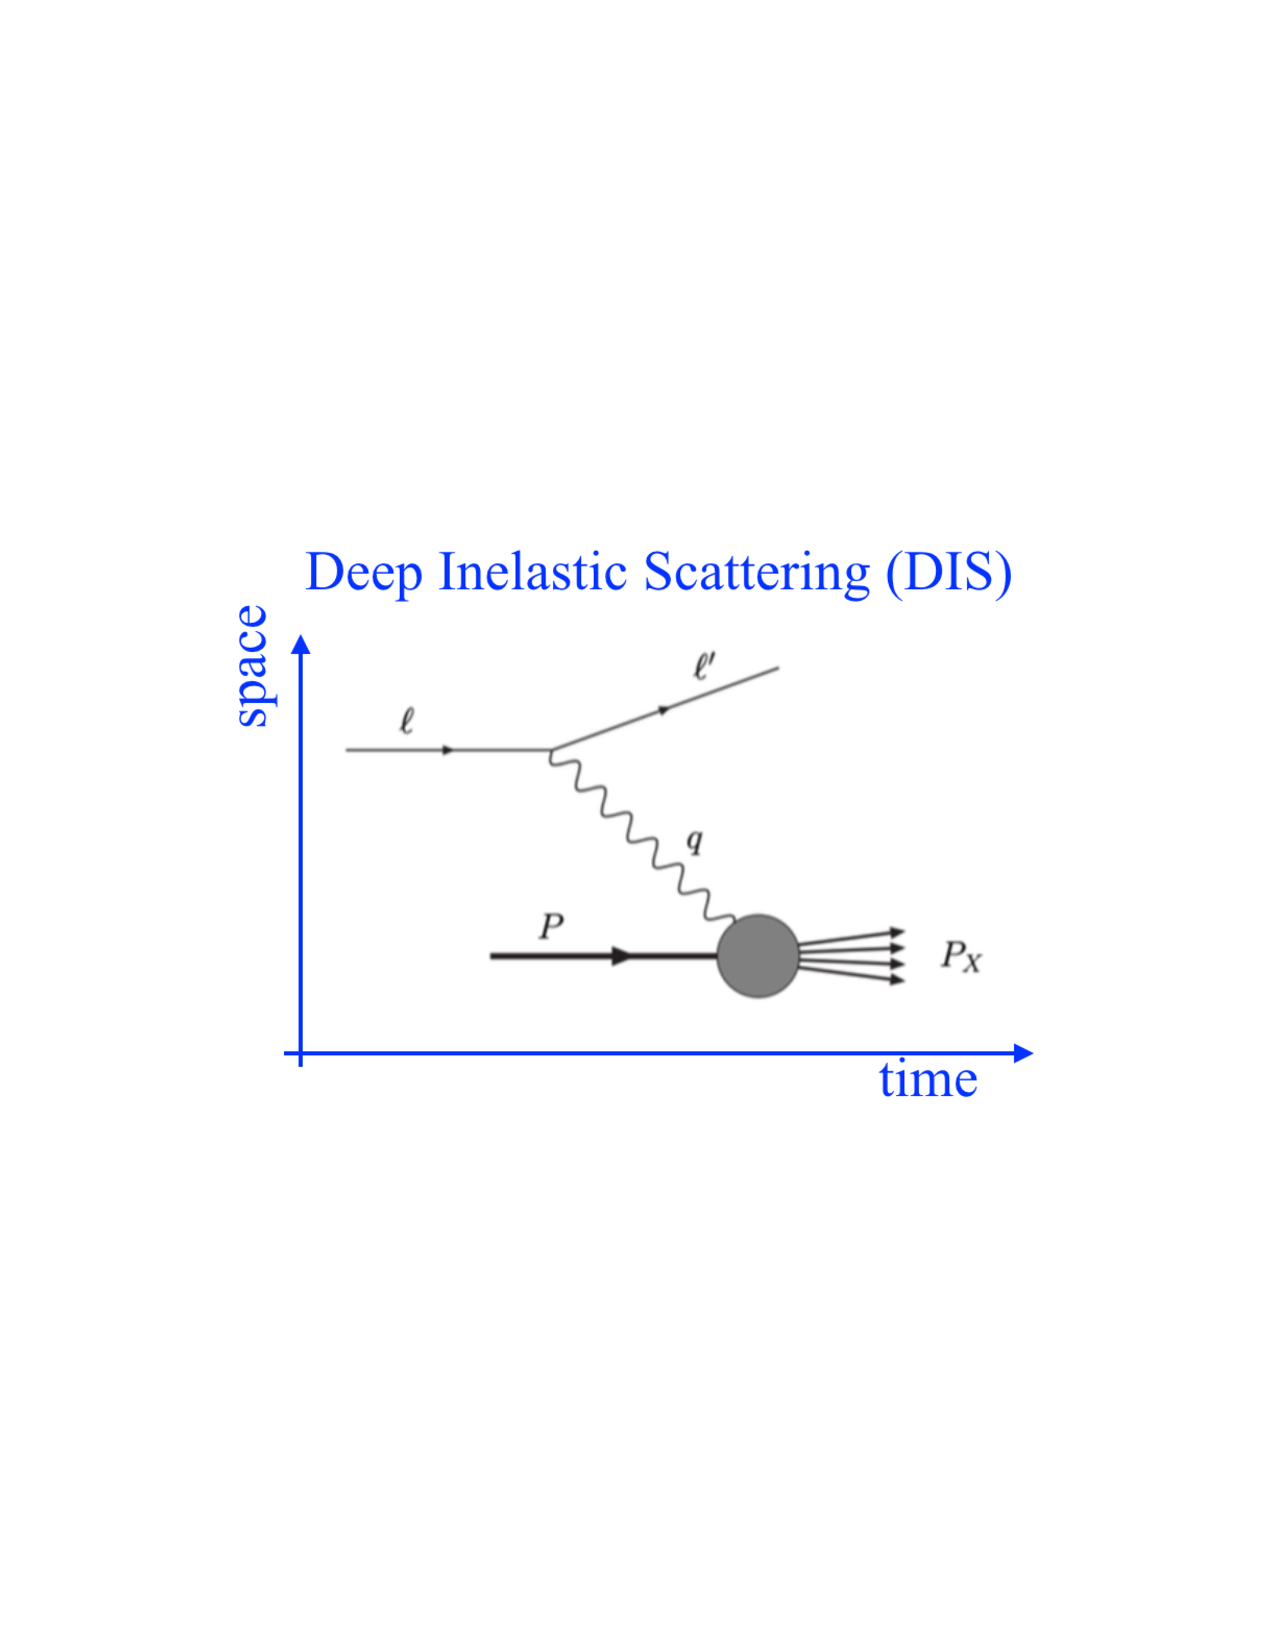
\includegraphics[width=0.7\textwidth, trim=4cm 9cm 4cm 9cm, clip]
      {DISxSect}
    \end{figure}
    \column{0.6\textwidth}
    \begin{figure}
      \centering
      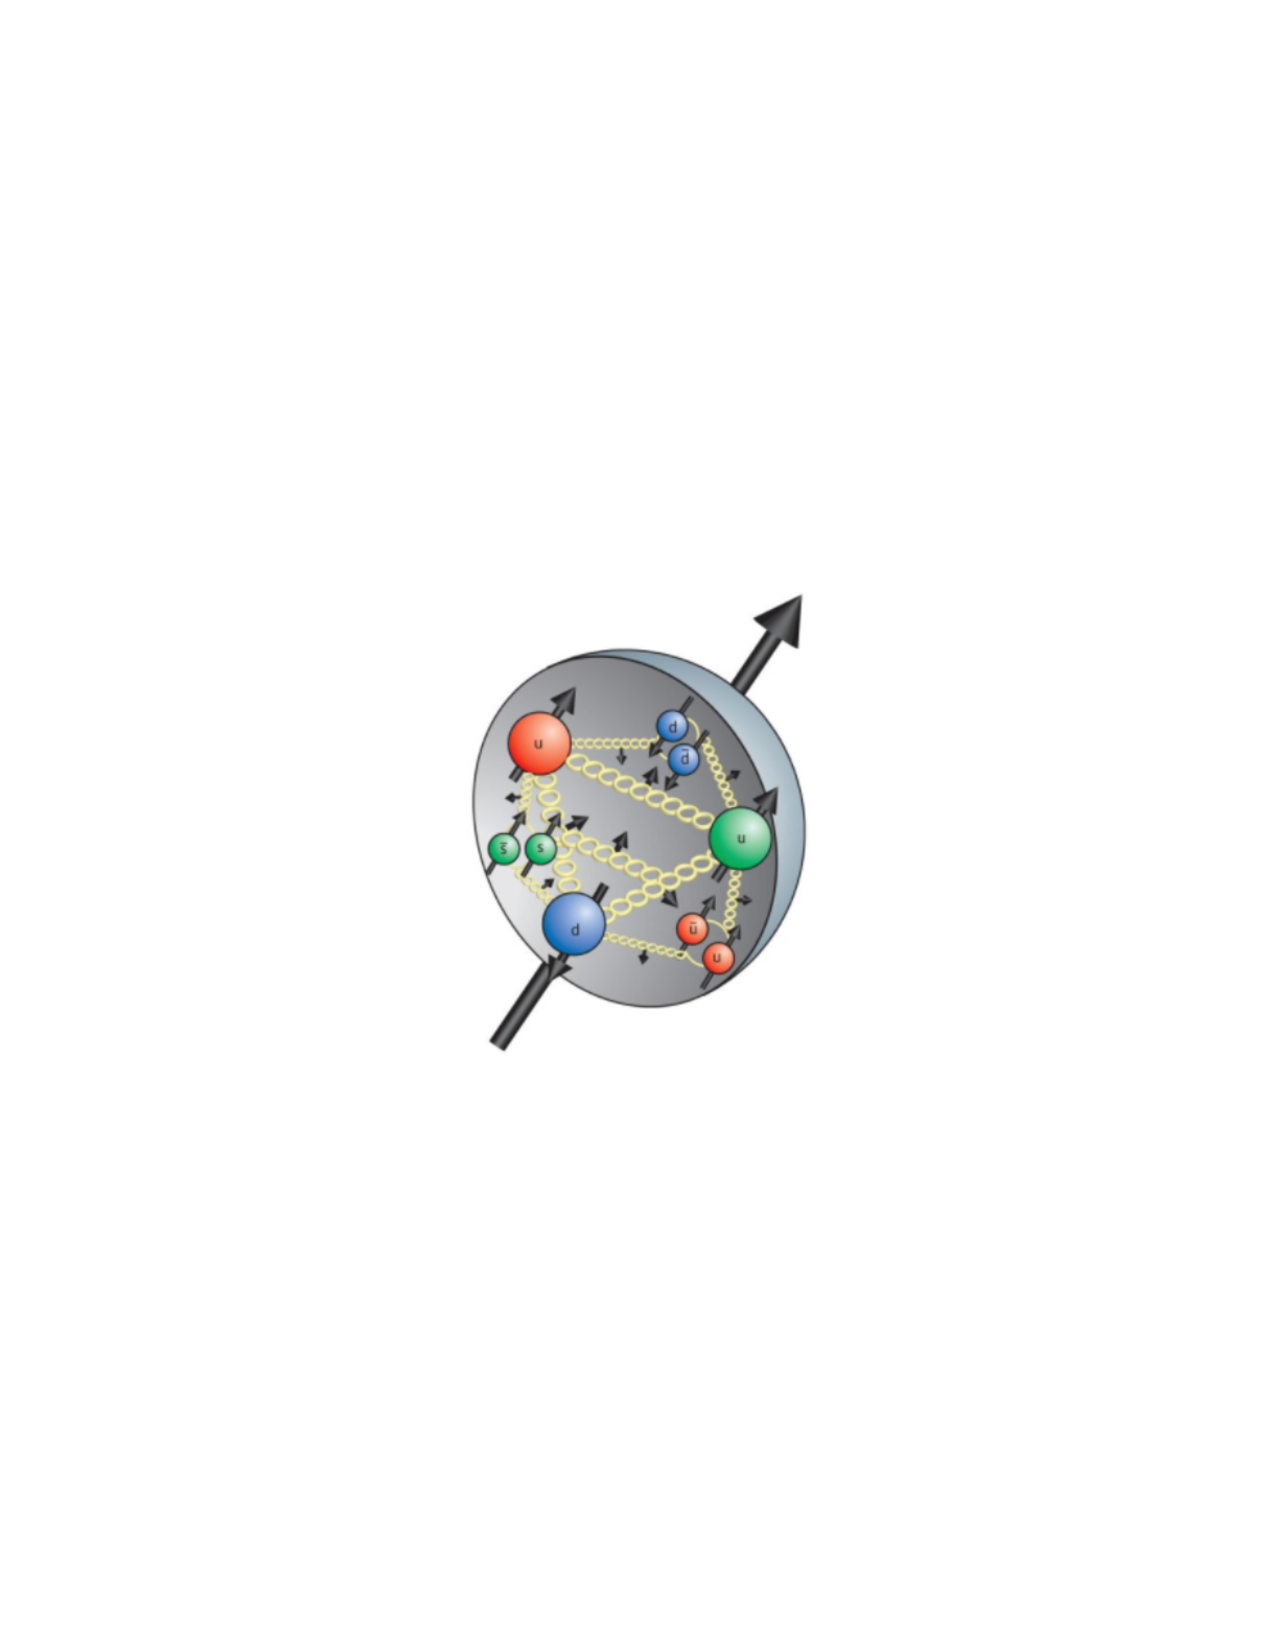
\includegraphics[width=0.7\textwidth, trim=7cm 10cm 7cm 10cm, clip]{Proton}
    \end{figure}
  \end{columns}

  \begin{itemize}
  \item Protons are made up of:
    \begin{itemize}
    \item up/up/down valence quarks (describe proton quantum numbers)
    \item sea quarks and gluons
    \end{itemize}
  \end{itemize}
  
\end{frame}


\begin{frame}
  \frametitle{Longitudinal Proton Spin Structure}

  \begin{columns}
    \column{0.47\textwidth}
    \setlength\abovecaptionskip{-5pt}
    \setlength{\belowcaptionskip}{-1pt}
    \begin{figure}
      \vspace*{-0.3cm}
      \centering
      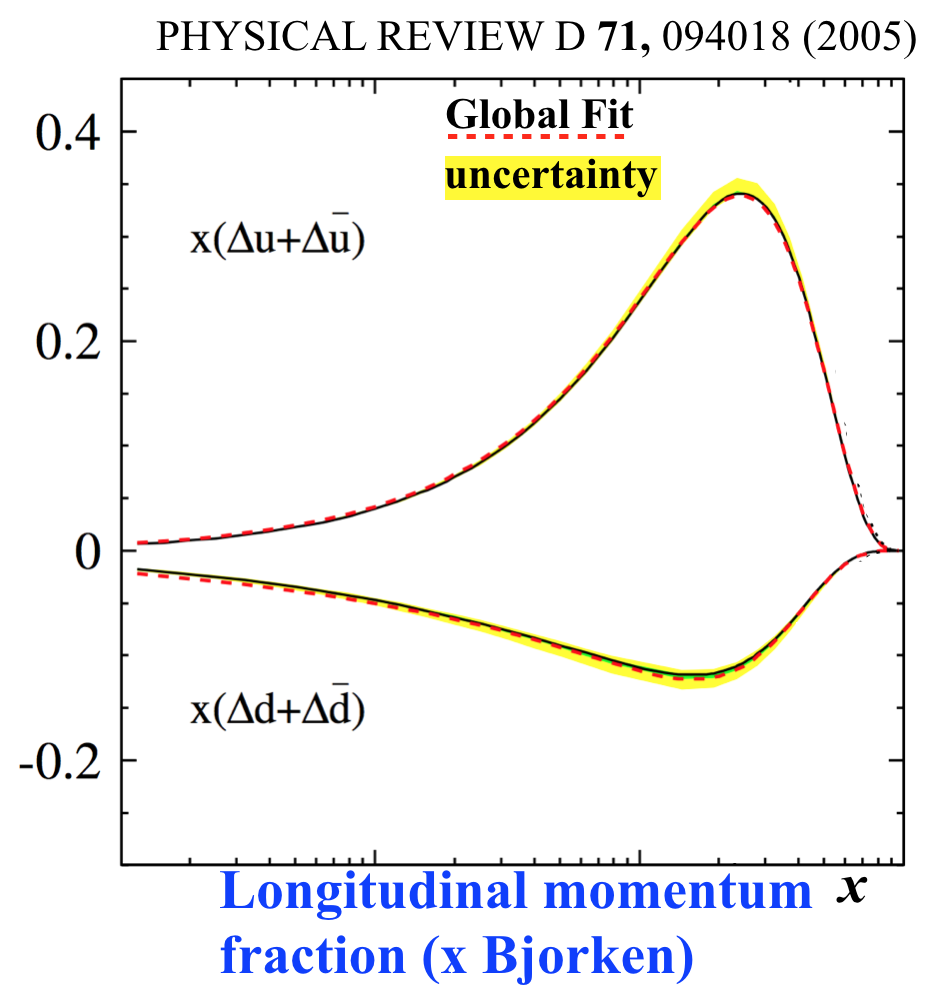
\includegraphics[width=\textwidth]{Helicity}
      \caption{Proton helicity distribution}
    \end{figure}
    \column{0.47\textwidth}
    \begin{dmath*}
      \Delta q = q^+ - q^- \\ \text{aligned quarks - anti-aligned quarks}
    \end{dmath*}
  \end{columns}
  
  \begin{itemize}
  \item Helicity distributions determined from $l^{\uparrow}+p^{\uparrow}
    \rightarrow l' + \pi + X$
  \item Integration gives the spin contribution from each quark flavor
  \end{itemize}
\end{frame}


\begin{frame}
  \frametitle{Transverse Proton Spin Structure}

  \begin{itemize}
  \item In a quark collinear approximation the quark transverse momentum should be small
    \begin{itemize}
    \item [] $\Rightarrow$ Analyzing power, A$_N$ = $\frac{1}{P}\frac{\sigma_{Left}^{\pi} - \sigma_{Right}^{\pi}}{\sigma_{Left}^{\pi} + \sigma_{Right}^{\pi}} \sim 10^{-4}$
    \end{itemize}
  \item E704 ($p^{\uparrow}+p\rightarrow \pi+X$) found much greater asymmetries   \end{itemize}

  \begin{figure}
    \centering
    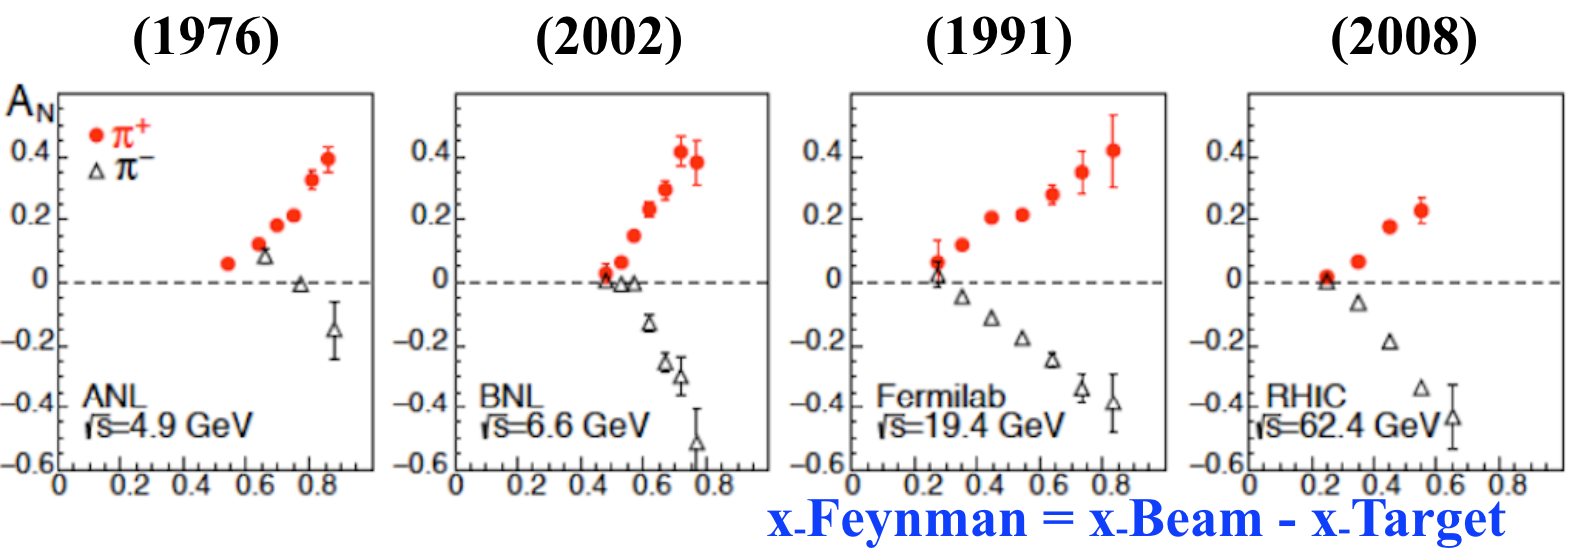
\includegraphics[width=\textwidth]{AN}
  \end{figure}
  \begin{itemize}
  \item A$_N$ is found large independent of the center of momentum energy
  \end{itemize}
\end{frame}


\begin{frame}
  \frametitle{Sivers Effect}

  \begin{itemize}
  \item One possible way to explain large single spin asymmetries
  \item Gives a correlation between proton transverse spin and transverse momentum of a parton
  \end{itemize}

  \setlength\abovecaptionskip{-5pt}
  \setlength{\belowcaptionskip}{-10pt}
  \begin{figure}
    \vspace*{-0.3cm}
    \centering
    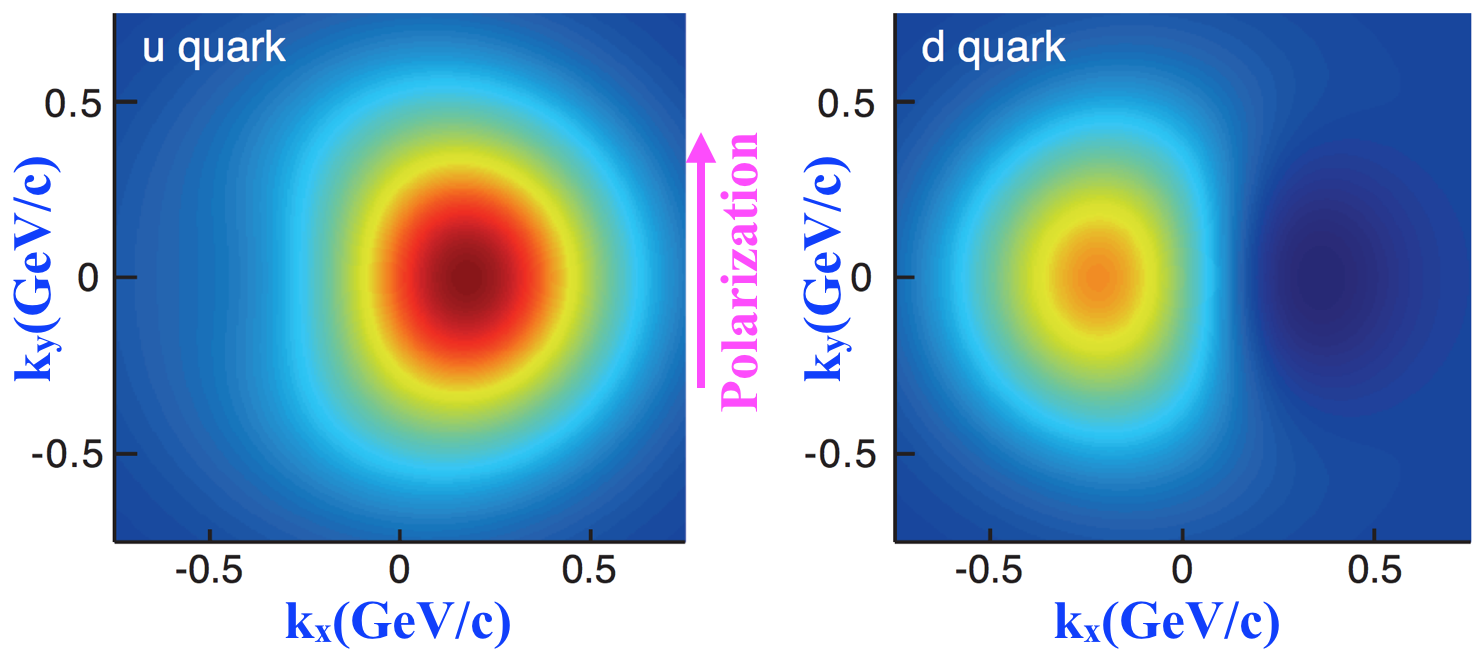
\includegraphics[width=0.7\textwidth]{SiversEffect}
    \caption{Lattice calculations of the quark transverse momentum in a polarized proton.}
  \end{figure}

  \begin{columns}
    \column{0.8\textwidth}
    \begin{itemize}
    \item Surprising result from theory: Sivers function is non-universal
    \item Expected to flip signs between
      \begin{itemize}
      \item [] $l+p^{\uparrow} \rightarrow l'+\pi+X$ and $h+p^{\uparrow} \rightarrow l+\bar{l}+X$
      \end{itemize}
    \end{itemize}
    \column{0.2\textwidth}
    \pause
    
\includegraphics[width=\textwidth]{NSFmilestone}
  \end{columns}
\end{frame}


\begin{frame}
  \frametitle{Sivers Measurement}

  \begin{itemize}
  \item COMPASS and HERMES measured a non-zero Sivers amplitude from
    semi-inclusive deep inelastic scattering (SIDIS)
    \begin{itemize}
      \item [] $l+p^{\uparrow} \rightarrow l'+h+X$
    \end{itemize}
  \end{itemize}

  \begin{figure}
    \centering
    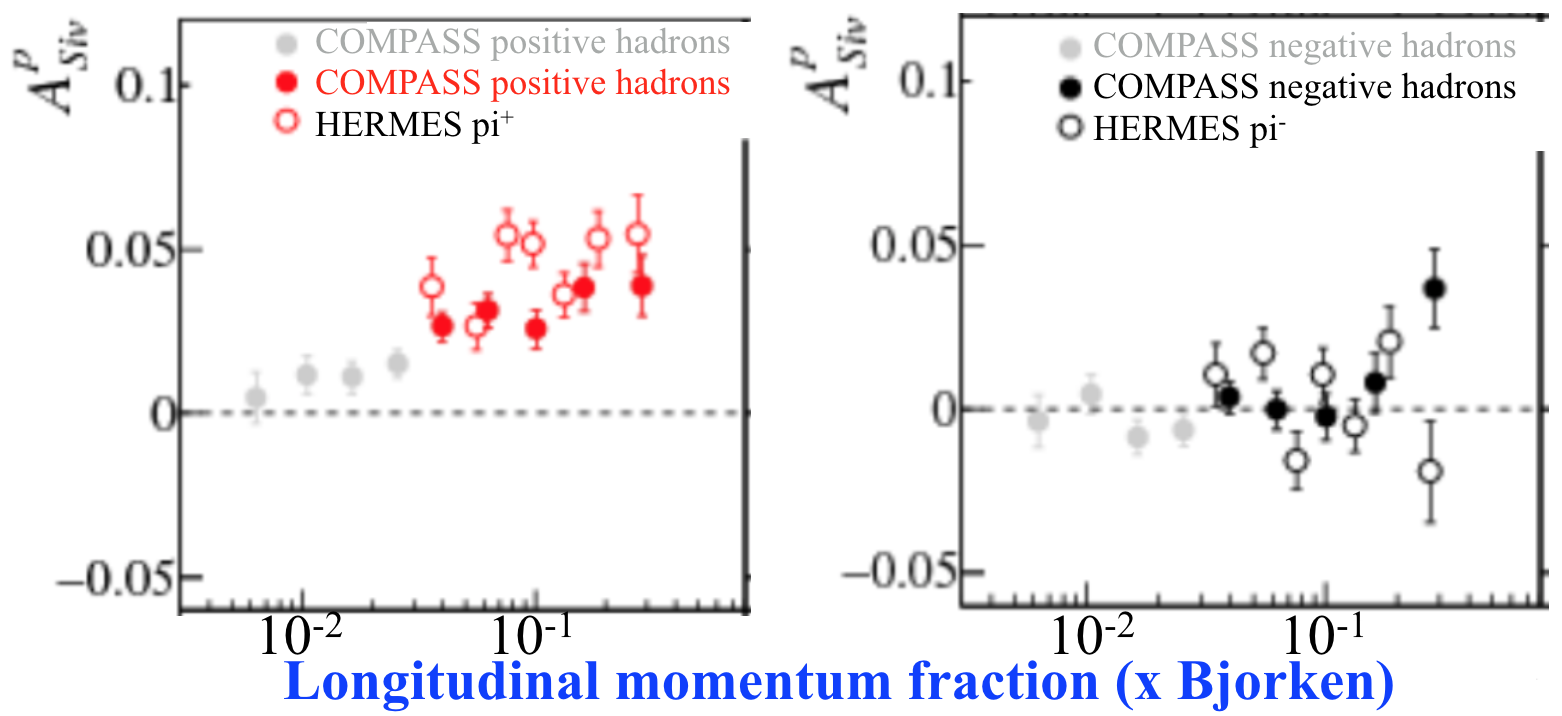
\includegraphics[width=0.95\textwidth]{SIDIS_siv}
    \caption{Sivers Amplitude related to the Sivers function}
  \end{figure}
\end{frame}


